\chapter{Discussion}\label{chap:conclusion}

\section{Evaluation of Results}
To summarize the research conducted up to this point, a GPU-supported parallel Andersen based pointer analysis, PTAGPU, was implemented on top of LLVM and the SVF framework using the NVIDIA CUDA SDK.
PTAGPU was both tested for correctness and performance in comparison to established CPU-based pointer analyses in multiple benchmarks and hardware combinations.
The primary research question was to what extent such an implementation presents advantages or disadvantages over other analyses that are not strictly parallel in nature.

The experimental results presented in \autoref{sec:results} indicate that PTAGPU is a viable implementation to improve the performance of a whole program field-sensitive pointer analysis without sacrificing precision of the analysis.
PTAGPU achieved an average speedup of 1.60 across 15 benchmarks over the SVF wavediff algorithm. Since the individual benchmarks with lower speedups are almost entirely smaller programs, the absolute time saved by using PTAGPU was 28 minutes and 59 seconds over the total 1 hour 07 minutes and 30 seconds required by wavediff to analyze the 15 benchmark programs. In terms of absolute time, the speedup factor was 1.75.
This represents a meaningful improvement over the CPU algorithm.
Unfortunately this does not include the Linux benchmark, as the analysis did not fit into graphics memory and did not finish within a reasonable amount of time, which was decided to be 24 hours.
Although enough total unified memory was available, the analysis of the Linux source code did become impeded by excessive page faults as illustrated in \autoref{sec:results}.
Judging from the wavediff analysis of the Linux kernel, roughly 300 GiB of memory are required for a successful whole program field-sensitive pointer analysis, which is currently impossible to compute entirely in the graphics memory of a single graphics card.

One key insight from the experimental results was, that there are no precise trivial prior indicators for analysis runtime, since the program structure is seemingly more influential on analysis runtime than lines of code, nodes in the constraint graph or size of the compiled program.
This is supported by prior research from \cite{mendez2012gpu} or \cite{su2015efficient}, where the selected benchmark programs - some of which overlap with the selected benchmark programs of this thesis - also had vastly different speedups for the GPU-based analysis over the CPU-based analyses.
It was found that the use of nested programming techniques, such as structures in a C program, can lead to a lower speedup on parallel hardware.
As a result, programs like git and the Linux kernel, that make extensive use of C structs, are performing worse in PTAGPU compared to other benchmark programs.
Because PTAGPU is field-sensitive, the effect of structures with fields in the source code disproportionately influences the runtime of the analysis compared to other instructions that can more easily be parallelized.
Still, the majority of benchmark programs did profit from the parallel analysis in PTAGPU and performed better on the GPU than on the CPU.

Although the results indicate that PTAGPU generally outperforms the CPU counterparts in larger benchmarks, it should be acknowledged that it is difficult to establish a fair comparison between CPU and GPU pointer analysis implementations.
Both in terms of upfront cost and power consumption both implementations are vastly different. While the SVF wavediff algorithm can be executed on almost any modern computer with sufficient system memory, PTAGPU requires specialized hardware. Especially for larger analyses, a GPU with enough graphics memory is required for an efficient analysis with PTAGPU.

\subsubsection{Comparing PTAGPU Results to other GPU-based implementations.}
Some other GPU-based Andersen style pointer analyses are \cite{mendez2012gpu} and \cite{su2015efficient}.
Unfortunately the results from both these GPU-based pointer analysis algorithms are not directly comparable with PTAGPU in terms of total runtime, since the reported constraint graph sizes are vastly smaller than those produced by SVF, indicating that they are incomplete in some way. Intuitively the reported result for performing a whole program field-sensitive inclusion-based pointer analysis on the Linux kernel in under ten seconds \cite{su2015efficient} does seem too fast, given the results from SVF.
Although the input data generation for these analyses was based on LLVM, according to a previous paper by Mendez et al. \cite{mendez2010parallel}, the source code for the data generation is not available.
Furthermore, indirect call-sites were not resolved during either of these analyses making them fundamentally incompatible with the results of PTAGPU.
Because the source code of neither of these implementations is available online and no other GPU-based implementations of Andersen style pointer analyses are known at this time, direct comparisons with other GPU implementations are omitted from the evaluation.

\section{Future Work}
During the development of PTAGPU and evaluation of the results, multiple novel approaches and ideas were discovered but not implemented, which will be summarized in the following section.
Some of these approaches could be used to further improve the performance of PTAGPU and alleviate shortcomings and limitations discovered during development.
Furthermore, some ideas could lead to improvements in the SVF project upstream, and inspire new research directions.

\subsubsection{Improvements for PTAGPU}
The hypothesized approach of using unified memory in a CUDA program to extend the scalability of PTAGPU and get around the limitation of only using the device's graphics memory did not work during experimental testing.
It was still necessary that the GPU had enough graphics memory to hold the entire analysis, because the performance of the algorithm would drastically decrease if graphics memory were to be exhausted while the analysis was still running. The reason for this was that accessing sparse bit vector elements outside of graphics memory would result in page faults and require moving the requested memory region into graphics memory, replacing a previous section of memory and slowing down the analysis.
The CUDA API does provide functions to prevent this behavior. By using \verb|cudaMemAdvise| and \verb|cudaMemPrefetchAsync| the developer can give hints to the memory controller as to where specific memory regions are preferred to be stored and loaded into before the data is actually required by the algorithm.
Fundamentally the problem with prefetching memory is the irregularity of a pointer analysis, making it very difficult to predict which memory regions are required in each iteration of the algorithm.

One possible solution to this problem would be a partitioning strategy, where the entire constraint graph is divided into roughly equally sized partitions.
The algorithm would then load each partition into device memory and resolve all constraints  $x \rightarrow y \rightarrow z \mathrel{\leadsto} x \rightarrow z$ where all nodes, x, y and z are included in the currently loaded partition.
To solve constraints that require loading nodes outside the current partition, two partitions are always loaded into memory in pairs. Constraints that involve nodes of both partitions are then solved. This is repeated until all constraints are resolved.
This exact approach was used by Graspan in \cite{zuo2021systemizing} using the file system instead of unified memory. The idea remains the same.

Developing a partitioning system instead of loading the entire constraint graph into graphics memory, would also enable the use of multiple GPUs without having to synchronize access to individual nodes across all devices.
The downside with partitioning the constraint graph lies in the fact that with an increasing number of partitions, the overhead associated with loading and unloading partitions increases.
Splitting the constraint graph into 16 partitions would require loading and unloading all 15 adjacent partitions in order to resolve all constraints of a single partition in the worst case.
Part of this problem can be reduced by performing an offline analysis and associating nodes with partitions such that a minimal number of edges overlap between partitions, leading to an optimal distribution of nodes for parallel graph rewriting.

Other than partitioning the constraint graph, there are various optimizations proposed in \cite{mendez2012gpu} that did not yield any immediate performance improvements during the development of PTAGPU but might bring improvements given more thorough testing.
These optimizations include online cycle detection and pointer-equivalent variable detection on the GPU during analysis.
Variables are pointer-equivalent if they possess the same outgoing points-to edges. These might be interesting to find, since applying a copy rewrite rule associated with any of the pointer-equivalent variables, results in the same operation on the GPU and would be redundant.
Similarly, a cycle of copy edges in the constraint graph would always hold the same points-to edges for each node in the cycle and thus should be detected during analysis to prevent redundant work.

Another approach for improving the scalability of PTAGPU would be the use of peer-to-peer memory access.
Peer-to-peer memory access is a capability of certain NVIDIA GPUs whereby multiple graphics cards can pool their memory though special NVLink interconnects on the GPUs, bypassing the bandwidth restrictions of the PCIe connections.
This would allow one kernel on a single device to access the graphics memory of several graphics cards and increase the available amount of memory during analysis and improving the scalability.

Finally, PTAGPU would greatly benefit from dynamic memory allocation. Currently, the total amount of unified memory has to be set during compilation, which is then allocated during runtime.
Since pointer analyses are very irregular calculations, it is very difficult to set the correct amount of memory before the analysis is run.
For this reason a dynamic memory allocation algorithm could improve the usability of PTAGPU by predicting and reallocating the amount of memory needed for the analysis.

\subsubsection{Improvements for SVF}
As PTAGPU and prior work has shown, there are lots of possibilities for parallelizing a pointer analysis.
Since GPUs are not the only devices capable of parallel execution, it would be another interesting avenue of research to apply some of the techniques discussed in this thesis on the CPU-based pointer analyses of SVF.
Seeing how other papers, like \cite{mendez2012gpu}, compared GPU and CPU parallel pointer analysis implementations, it would be interesting to compare a parallelized SVF-based pointer analysis on the CPU to PTAGPU. Especially for smaller programs, this might bring performance improvements.
Part of a parallel CPU implementation in SVF would be to create thread safe versions of the internal SVF data structures.
This would also indirectly improve the performance of PTAGPU, since the asynchronous CPU section of PTAGPU also utilizes parts of SVF that currently can not be parallelized.
Especially improving the parallel resolution of \verb|getelementpointer| constraints could yield great improvements for PTAGPU, since dealing with nested code structures is currently one of its weaknesses.
It would also be interesting to further analyze the effects of using specific language constructs on the runtime performance on parallel pointer analyses.

Ultimately it would be a good idea to implement a hybrid pointer analysis in SVF that would be capable of utilizing both CPUs and GPUs for the analysis depending on the program to be analyzed.
Using the CPU implementation for smaller programs and the GPU implementation for larger programs until graphics memory is exhausted, could maximize the performance for different kinds of input programs.
Since pointer analyses do not remove any already computed points-to data, a given analysis could switch between CPU and GPU implementations relatively uninterruptedly, without having to repeat a large amount of work.
Using diffpoints further improves this process.

Finally, another avenue for future research is the reevaluation of context-free-grammars, possibly in a parallel execution environment, for the purpose of pointer analysis.
Recent additions to the SVF framework include a solver component that explicitly utilizes context-free-grammars \cite{lei2022taming} and is allegedly more performant than Graspan at querying CFL-reachability in a graph, according to the cited paper.
\section{Conclusion}
Concluding, PTAGPU was capable of meaningfully improving the performance of a whole program field-sensitive pointer analysis on top of LLVM and the SVF framework.
The main advantages lie with relatively large programs that are built using a relatively flat code structure, where PTAGPU achieves a respectable speedup over CPU-based pointer analyses.
Given how general Andersen style pointer analyses are a P-complete computational problem \cite{mathiasen2021fine}, this result is not achieved by trivial methods, but requires a wide set of complex analysis techniques and optimizations. All while being able to use a reproducible and well-defined input format in the form of LLVM bitcode.

The main disadvantages are that using GPUs for a pointer analysis always introduces an overhead for graphics memory management and conversion of input data into a format suitable for the GPU.
This makes using GPUs for analyzing small programs (less than 1 MB in size) inefficient.
For optimal performance PTAGPU also requires that the entire analysis fits into graphics memory, which currently prevents some of the largest software projects, such as the Linux kernel, from being analyzed by PTAGPU efficiently.

Overall the parallel GPU-based pointer analysis PTAGPU has shown to be a promising approach for improving the efficiency of pointer analysis. By leveraging the parallel processing capabilities of GPUs, PTAGPU was able to achieve an average speedup of 1.60 over the state-of-the-art wavediff pointer analysis in the SVF framework. This demonstrates the potential of PTAGPU to significantly reduce the time required for pointer analysis, making it a valuable tool for developers and researchers working in this field.
This implementation should provide a good reference for future research into parallel pointer analyses and can easily be expanded upon based on the modular design of the SVF framework.
\appendix

\chapter{Raw Data}

\begin{table}[ht]
    \tiny
    \begin{tabular}{rrrrrrrrr}
        \toprule
        id & file         & GPU memory MiB & filesize MB & wavediff-t   & naiveander-t & \# nodes & \# edges & version \\
        \midrule
        1  & bash         & 1024           & 5.400       & 16222.113    & 102195.752   & 238      & 77       & 5.1.16  \\
        2  & bison        & 260            & 3.400       & 18977.376    & 119999.054   & 146      & 59       & 3.8     \\
        3  & diff         & 71             & 1.300       & 1469.056     & 1561.577     & 54       & 17       & 3.8     \\
        4  & git          & 21467          & 25.000      & 557953.924   & 33404492.853 & 869      & 379      & 2.37.4  \\
        5  & htop         & 93             & 1.600       & 2912.693     & 5696.107     & 48       & 20       & 3.2.1   \\
        6  & httpd        & 160            & 1.400       & 5321.631     & 2889.208     & 169      & 95       & 2.4.54  \\
        7  & nano         & 7              & 0.298       & 87.438       & 98.500       & 6        & 2        & 6.4     \\
        8  & perl         & 3999           & 4.900       & 103338.824   & 2688610.846  & 445      & 206      & 5.37.3  \\
        9  & php          & 27561          & 52.000      & 645697.175   & 6530636.248  & 1582     & 611      & 7.4.31  \\
        10 & postgres     & 16430          & 18.000      & 997355.718   & 6481597.401  & 1432     & 721      & 14.4    \\
        11 & python       & 9016           & 21.000      & 536515.479   & 1731373.999  & 742      & 313      & 3.10.6  \\
        12 & redis-server & 207            & 4.800       & 8679.144     & 4834.759     & 207      & 67       & 7.0.5   \\
        13 & vim          & 11966          & 7.700       & 1052995.525  & NaN          & 696      & 280      & 9.0     \\
        14 & vmlinux      & NaN            & 72.000      & 32100566.652 & NaN          & 4464     & 2206     & 5.14    \\
        15 & vmlinux-tiny & 2175           & 5.400       & 91479.697    & 1410004.628  & 393      & 157      & 5.14    \\
        16 & zstd         & 454            & 2.300       & 11063.214    & 7958.999     & 280      & 101      & 1.5.2   \\
        \bottomrule
    \end{tabular}

    \caption[Raw Data of Baseline results for wavediff and naive-ander Pointer Analyses]{Raw Data of Baseline results for wavediff and naive-ander Pointer Analyses\\Node and Edge count in thousands, times in ms.}
\end{table}

\begin{table}[ht]
    \tiny
    \begin{tabular}{rrrrrrrrrr}
        \toprule
        id & ptagpu-t    & svf init & cuda init & update-k   & main-k       & thrust sort & store-k      & async CPU  & S    \\
        \midrule
        1  & 15489.00    & 366.515  & 2489.389  & 1129.063   & 1324.698     & 743.670     & 858.932      & 5190.693   & 1.05 \\
        2  & 9837.06     & 214.357  & 1650.840  & 830.177    & 234.046      & 675.748     & 54.633       & 4317.114   & 1.93 \\
        3  & 4231.58     & 66.945   & 2065.479  & 103.057    & 33.120       & 379.843     & 23.591       & 953.283    & 0.35 \\
        4  & 4690010.00  & 2190.250 & 17095.315 & 70148.000  & 3968158.215  & 11743.372   & 68373.295    & 538454.710 & 0.12 \\
        5  & 5275.51     & 68.425   & 2053.573  & 229.714    & 202.955      & 433.321     & 41.092       & 1587.968   & 0.55 \\
        6  & 6414.69     & 309.354  & 1481.509  & 303.996    & 42.605       & 511.057     & 8.219        & 1637.408   & 0.83 \\
        7  & 1751.01     & 7.732    & 1533.113  & 1.829      & 3.040        & 45.140      & 1.057        & 94.275     & 0.05 \\
        8  & 45093.40    & 775.915  & 2939.635  & 3457.350   & 6125.819     & 767.334     & 2751.206     & 21457.059  & 2.29 \\
        9  & 64965400.00 & 2809.670 & 20928.407 & 193679.543 & 53783100.092 & 12298.489   & 10732741.786 & 187398.213 & 0.01 \\
        10 & 465527.00   & 2911.590 & 8824.470  & 65379.251  & 192989.575   & 1374.555    & 32019.477    & 135372.093 & 2.14 \\
        11 & 203649.00   & 1344.910 & 4088.639  & 14380.164  & 63762.440    & 16295.704   & 12199.745    & 79598.063  & 2.63 \\
        12 & 11592.50    & 357.262  & 2785.032  & 688.684    & 95.318       & 1158.755    & 42.613       & 3688.319   & 0.75 \\
        13 & 268628.00   & 1166.830 & 9292.169  & 10709.775  & 113872.762   & 947.744     & 20876.445    & 100689.414 & 3.92 \\
        14 & NaN         & NaN      & NaN       & NaN        & NaN          & NaN         & NaN          & NaN        & NaN  \\
        15 & 188315.00   & 654.966  & 2405.784  & 10600.173  & 25890.805    & 12319.814   & 7893.207     & 121492.773 & 0.49 \\
        16 & 13172.60    & 388.764  & 2791.627  & 680.571    & 90.320       & 687.799     & 80.554       & 4526.521   & 0.84 \\
        \bottomrule
    \end{tabular}
    \caption{Raw Data of PTAGPU on Machine B, times in ms}
\end{table}

\begin{table}[ht]
    \tiny
    \begin{tabular}{rrrrrrrrrr}
        \toprule
        id & ptagpu-t   & svf init & cuda init & update-k  & main-k     & thrust sort & store-k   & async CPU  & S    \\
        \midrule
        1  & 13126.316  & 316.589  & 3339.273  & 955.132   & 1258.228   & 103.923     & 824.671   & 3404.405   & 1.23 \\
        2  & 7599.453   & 181.425  & 3397.507  & 657.559   & 203.553    & 92.256      & 41.323    & 2941.927   & 2.49 \\
        3  & 3304.592   & 53.196   & 3119.867  & 100.198   & 29.448     & 73.122      & 13.813    & 379.511    & 0.44 \\
        4  & 869302.000 & 1489.250 & 2852.620  & 31480.079 & 350891.929 & 4856.937    & 30923.576 & 431554.218 & 0.64 \\
        5  & 4038.684   & 58.770   & 3238.629  & 212.349   & 189.568    & 74.528      & 20.536    & 852.136    & 0.72 \\
        6  & 4720.701   & 233.173  & 3125.778  & 258.309   & 39.757     & 57.139      & 5.049     & 848.704    & 1.12 \\
        7  & 1626.456   & 5.655    & 3163.307  & 2.024     & 4.073      & 8.778       & 0.786     & 18.179     & 0.05 \\
        8  & 41853.936  & 644.417  & 3277.899  & 3452.222  & 6873.348   & 164.523     & 2906.182  & 18027.103  & 2.46 \\
        9  & 500086.000 & 2561.200 & 3815.678  & 32016.810 & 184075.139 & 2797.468    & 49062.434 & 198397.500 & 1.29 \\
        10 & 290219.000 & 2465.070 & 4439.149  & 12040.787 & 140270.103 & 211.504     & 14064.883 & 89735.395  & 3.43 \\
        11 & 172701.000 & 1088.500 & 3468.036  & 14790.821 & 65522.991  & 203.848     & 11336.972 & 63986.167  & 3.10 \\
        12 & 8830.066   & 247.339  & 3339.556  & 615.407   & 103.871    & 109.152     & 24.580    & 2143.869   & 0.98 \\
        13 & 247859.000 & 963.959  & 3336.741  & 7599.231  & 125708.265 & 123.820     & 23102.001 & 75995.761  & 4.24 \\
        14 & NaN        & NaN      & NaN       & NaN       & NaN        & NaN         & NaN       & NaN        & NaN  \\
        15 & 136164.602 & 554.447  & 3152.182  & 11286.157 & 26563.670  & 236.409     & 8721.936  & 79417.327  & 0.67 \\
        16 & 9795.036   & 312.077  & 3104.891  & 546.614   & 70.509     & 75.957      & 61.621    & 2587.828   & 1.12 \\
        \bottomrule
    \end{tabular}
    \caption{Raw Data of PTAGPU on Machine C, times in ms}
\end{table}
\normalsize

\begin{figure}[ht]
    \centering
    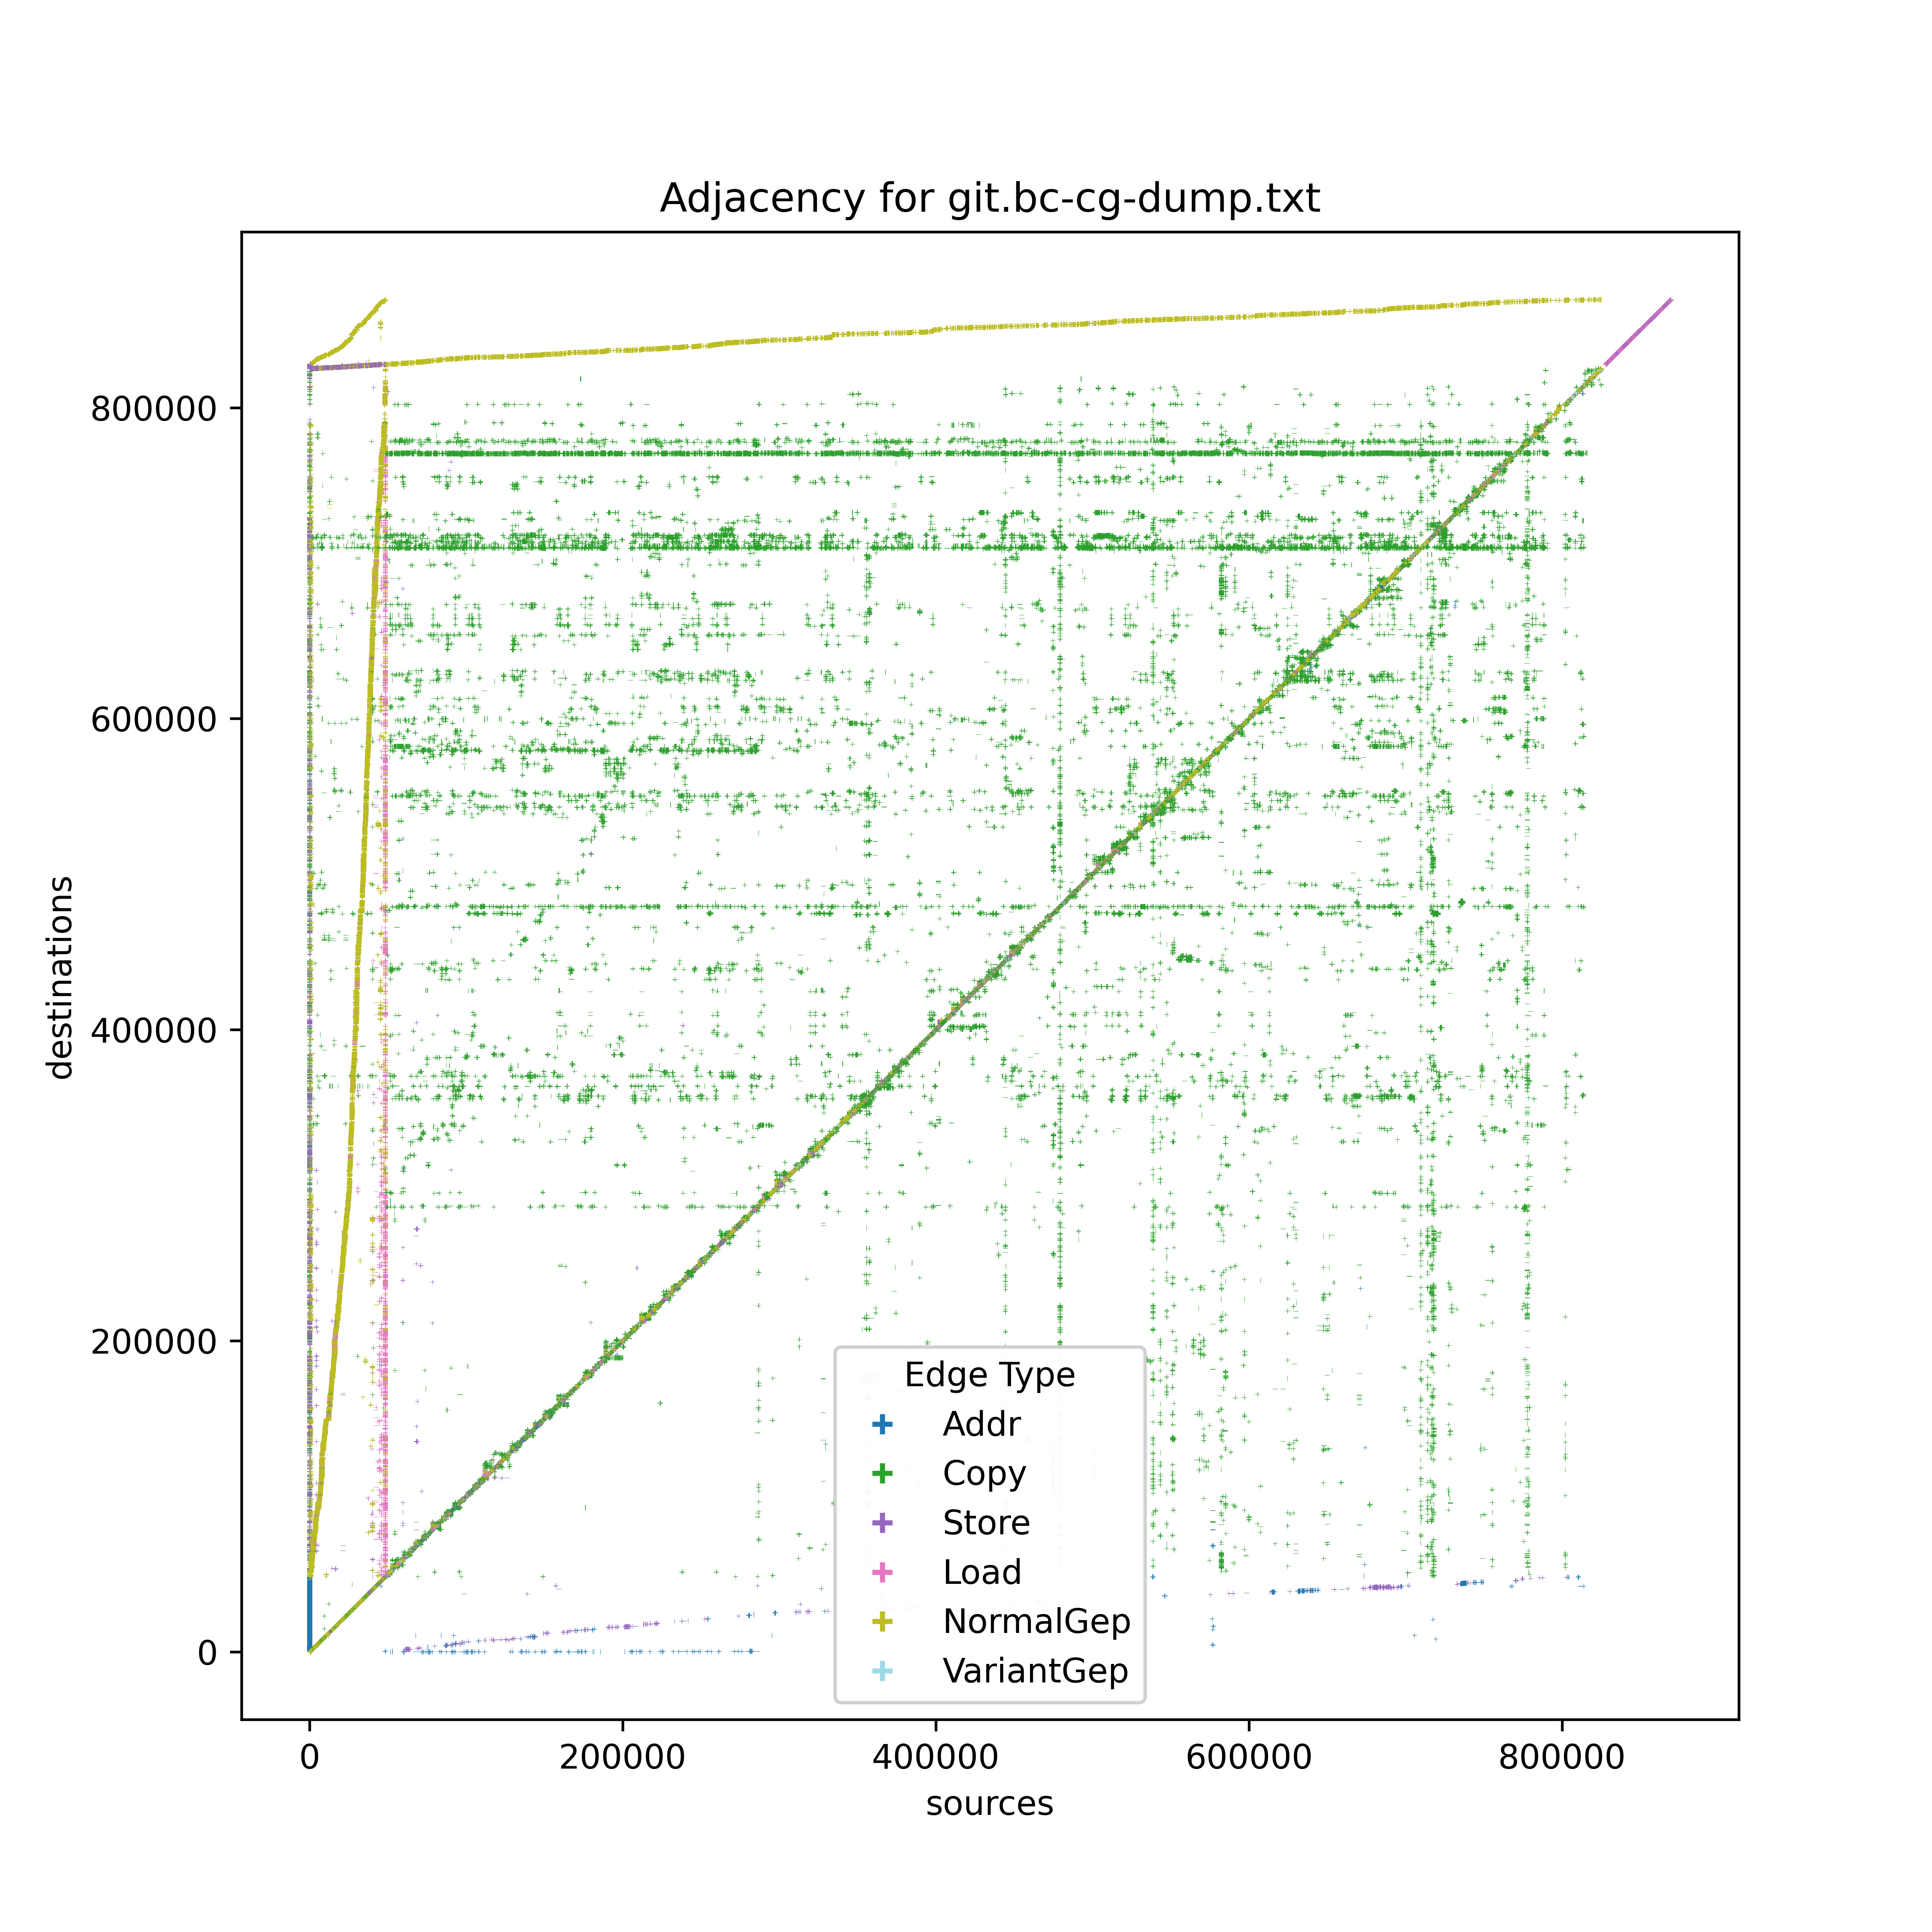
\includegraphics[width=1.\textwidth]{img/plot-git.bc-cg-dump.txt-min.png}
    \caption{Adjacency Plot for the Constraint Graph of the Git Client}
    \label{fig:git-consg}
\end{figure}

\begin{figure}[ht]
    \centering
    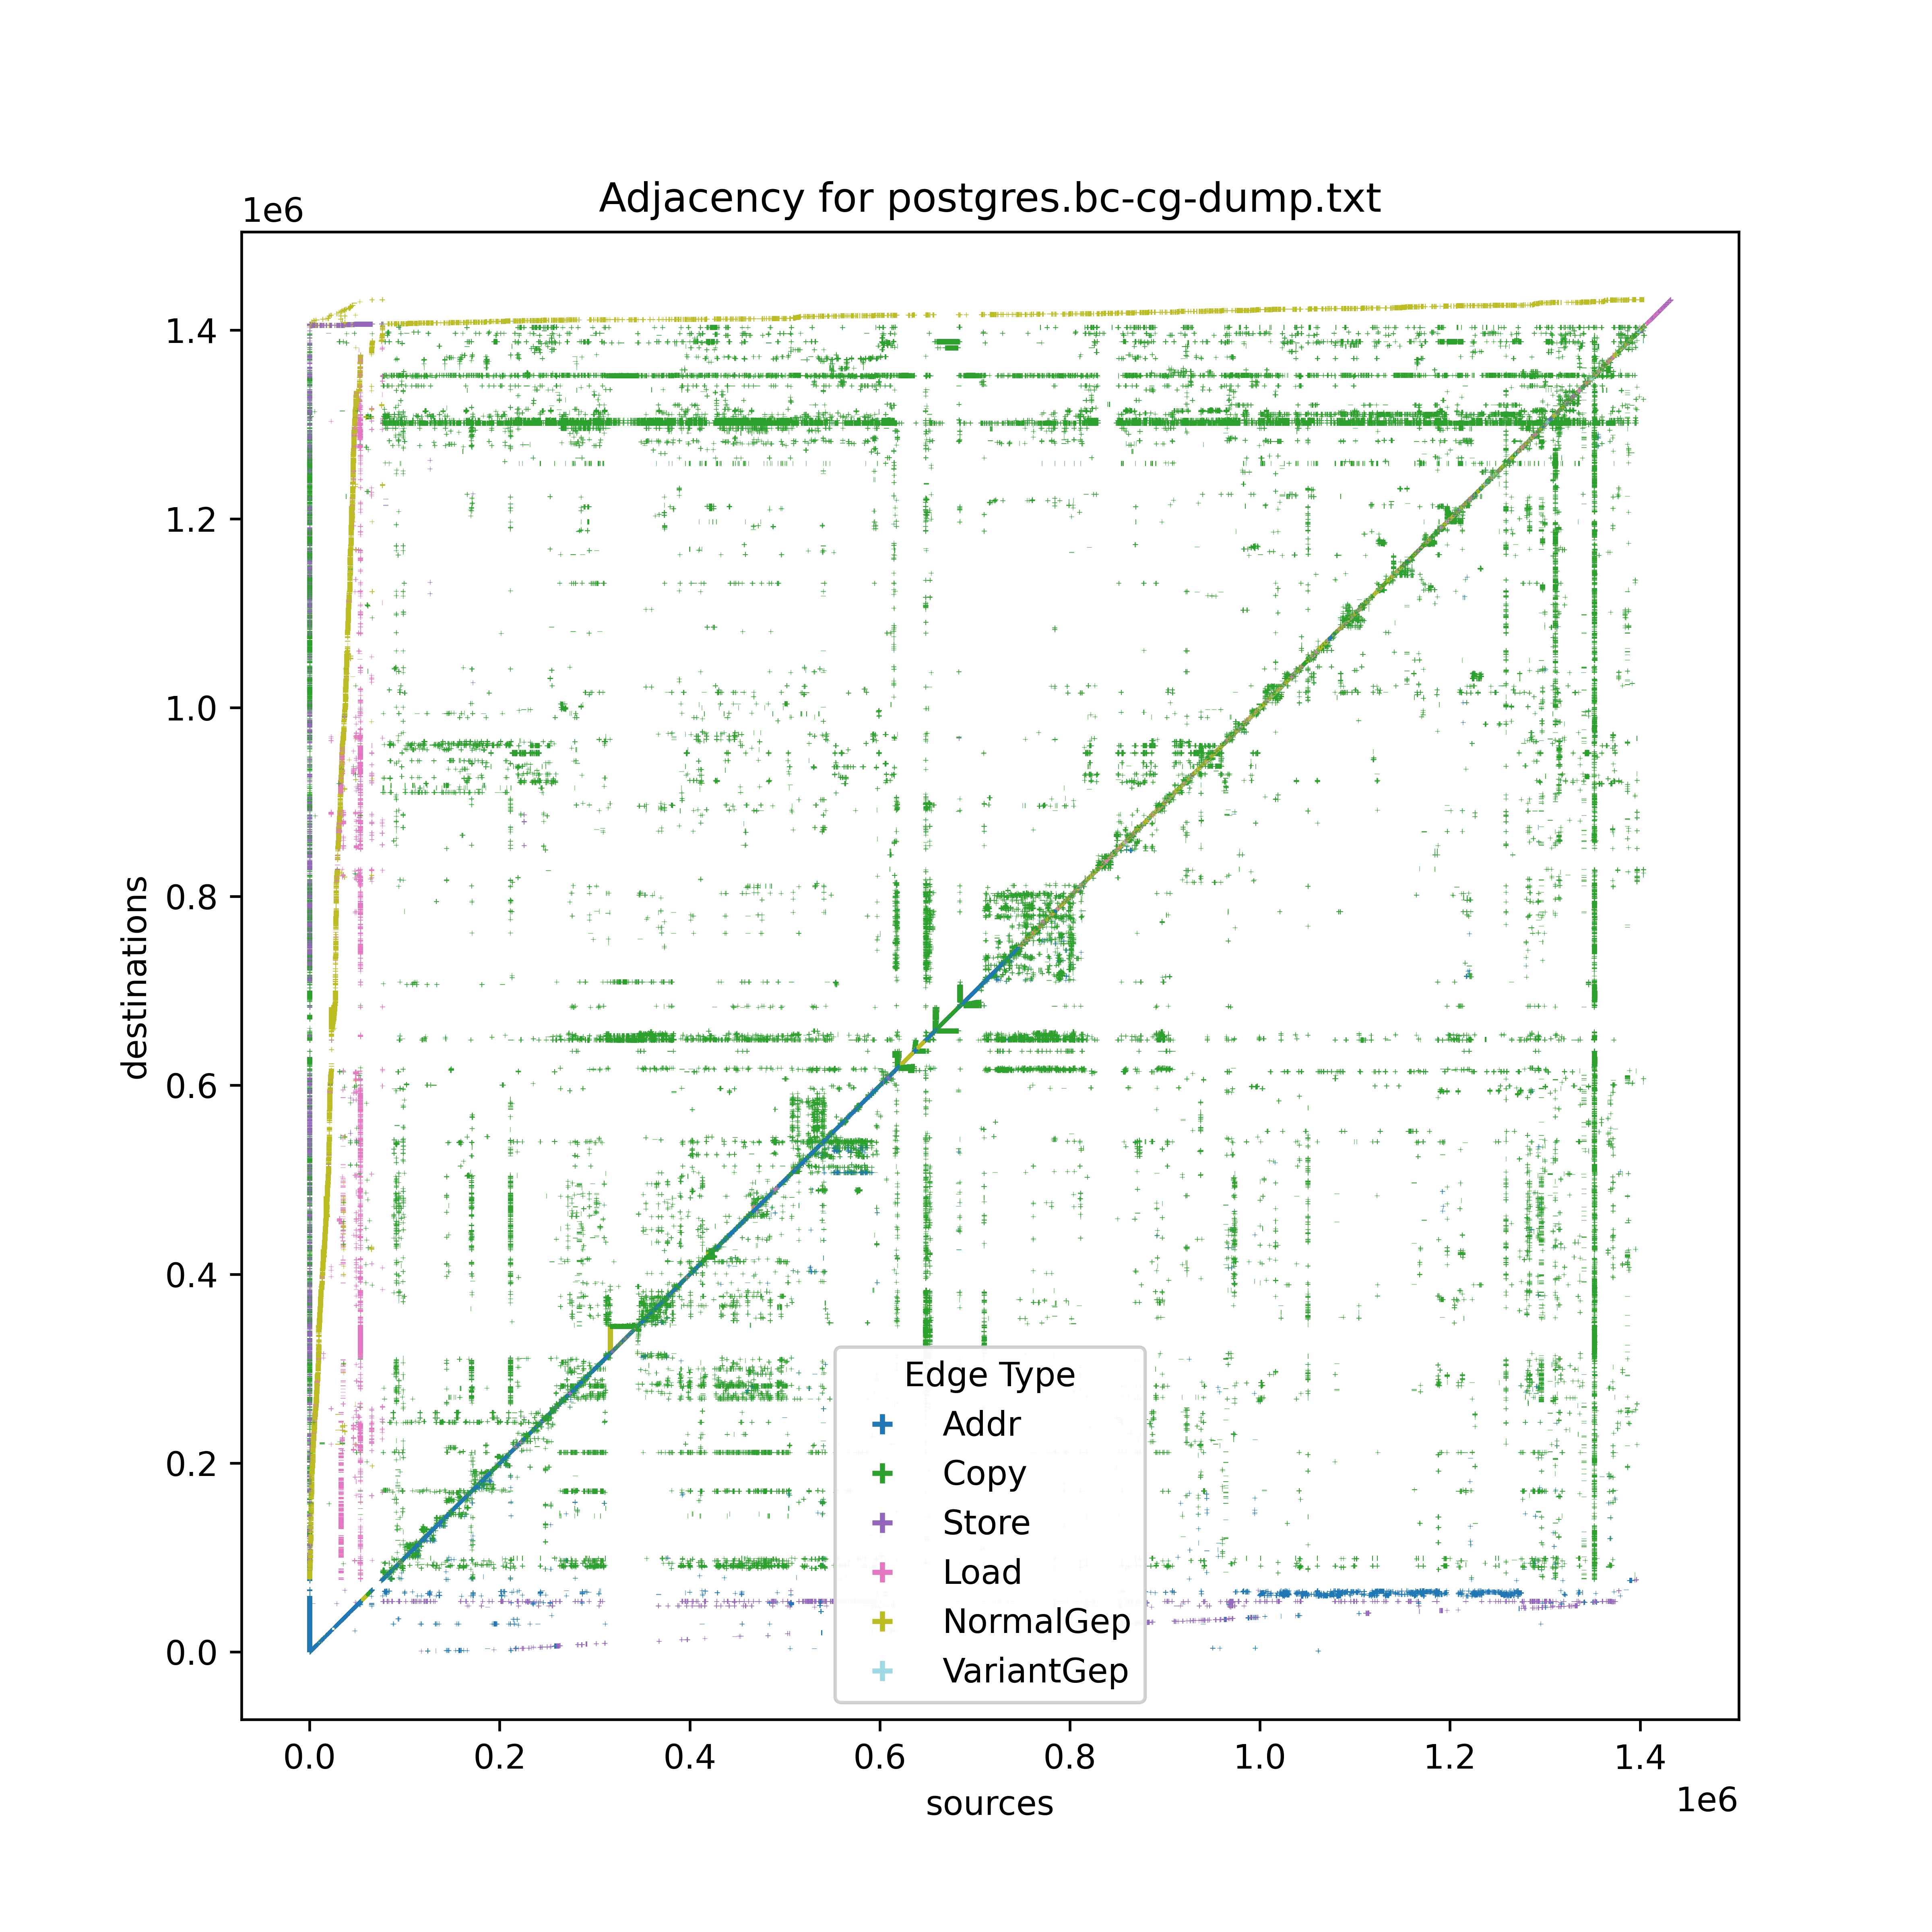
\includegraphics[width=1.\textwidth]{img/plot-postgres.bc-cg-dump.txt-min.png}
    \caption{Adjacency Plot for the Constraint Graph of Postgres}
    \label{fig:postgres-consg}
\end{figure}
